En esta sección concretamos en circuitos reales los conceptos abstractos de la sección anterior, justificando cada parte del circuito y la elección de sus componentes.
En la figura~\figref{fig:designed_circuit} puede verse nuestro circuito amplificador completo, incluyendo el punto de trabajo de cada transistor, es el circuito que se usó en cada una de las simulaciones para validar el circuito contra las especificaciones que se establecieron. En el circuito también se marcaron algunos ratings de componentes, potencias de resistores y tensiones de capacitores, los cuales se obtuvieron de las simulaciones, estos se especificaron y se usaron a la hora de armar el listado de componentes final, teniendo en cuenta también las tecnologías adecuadas para cada componente elegido.

\clearpage


\begin{figure}[H]
\centering
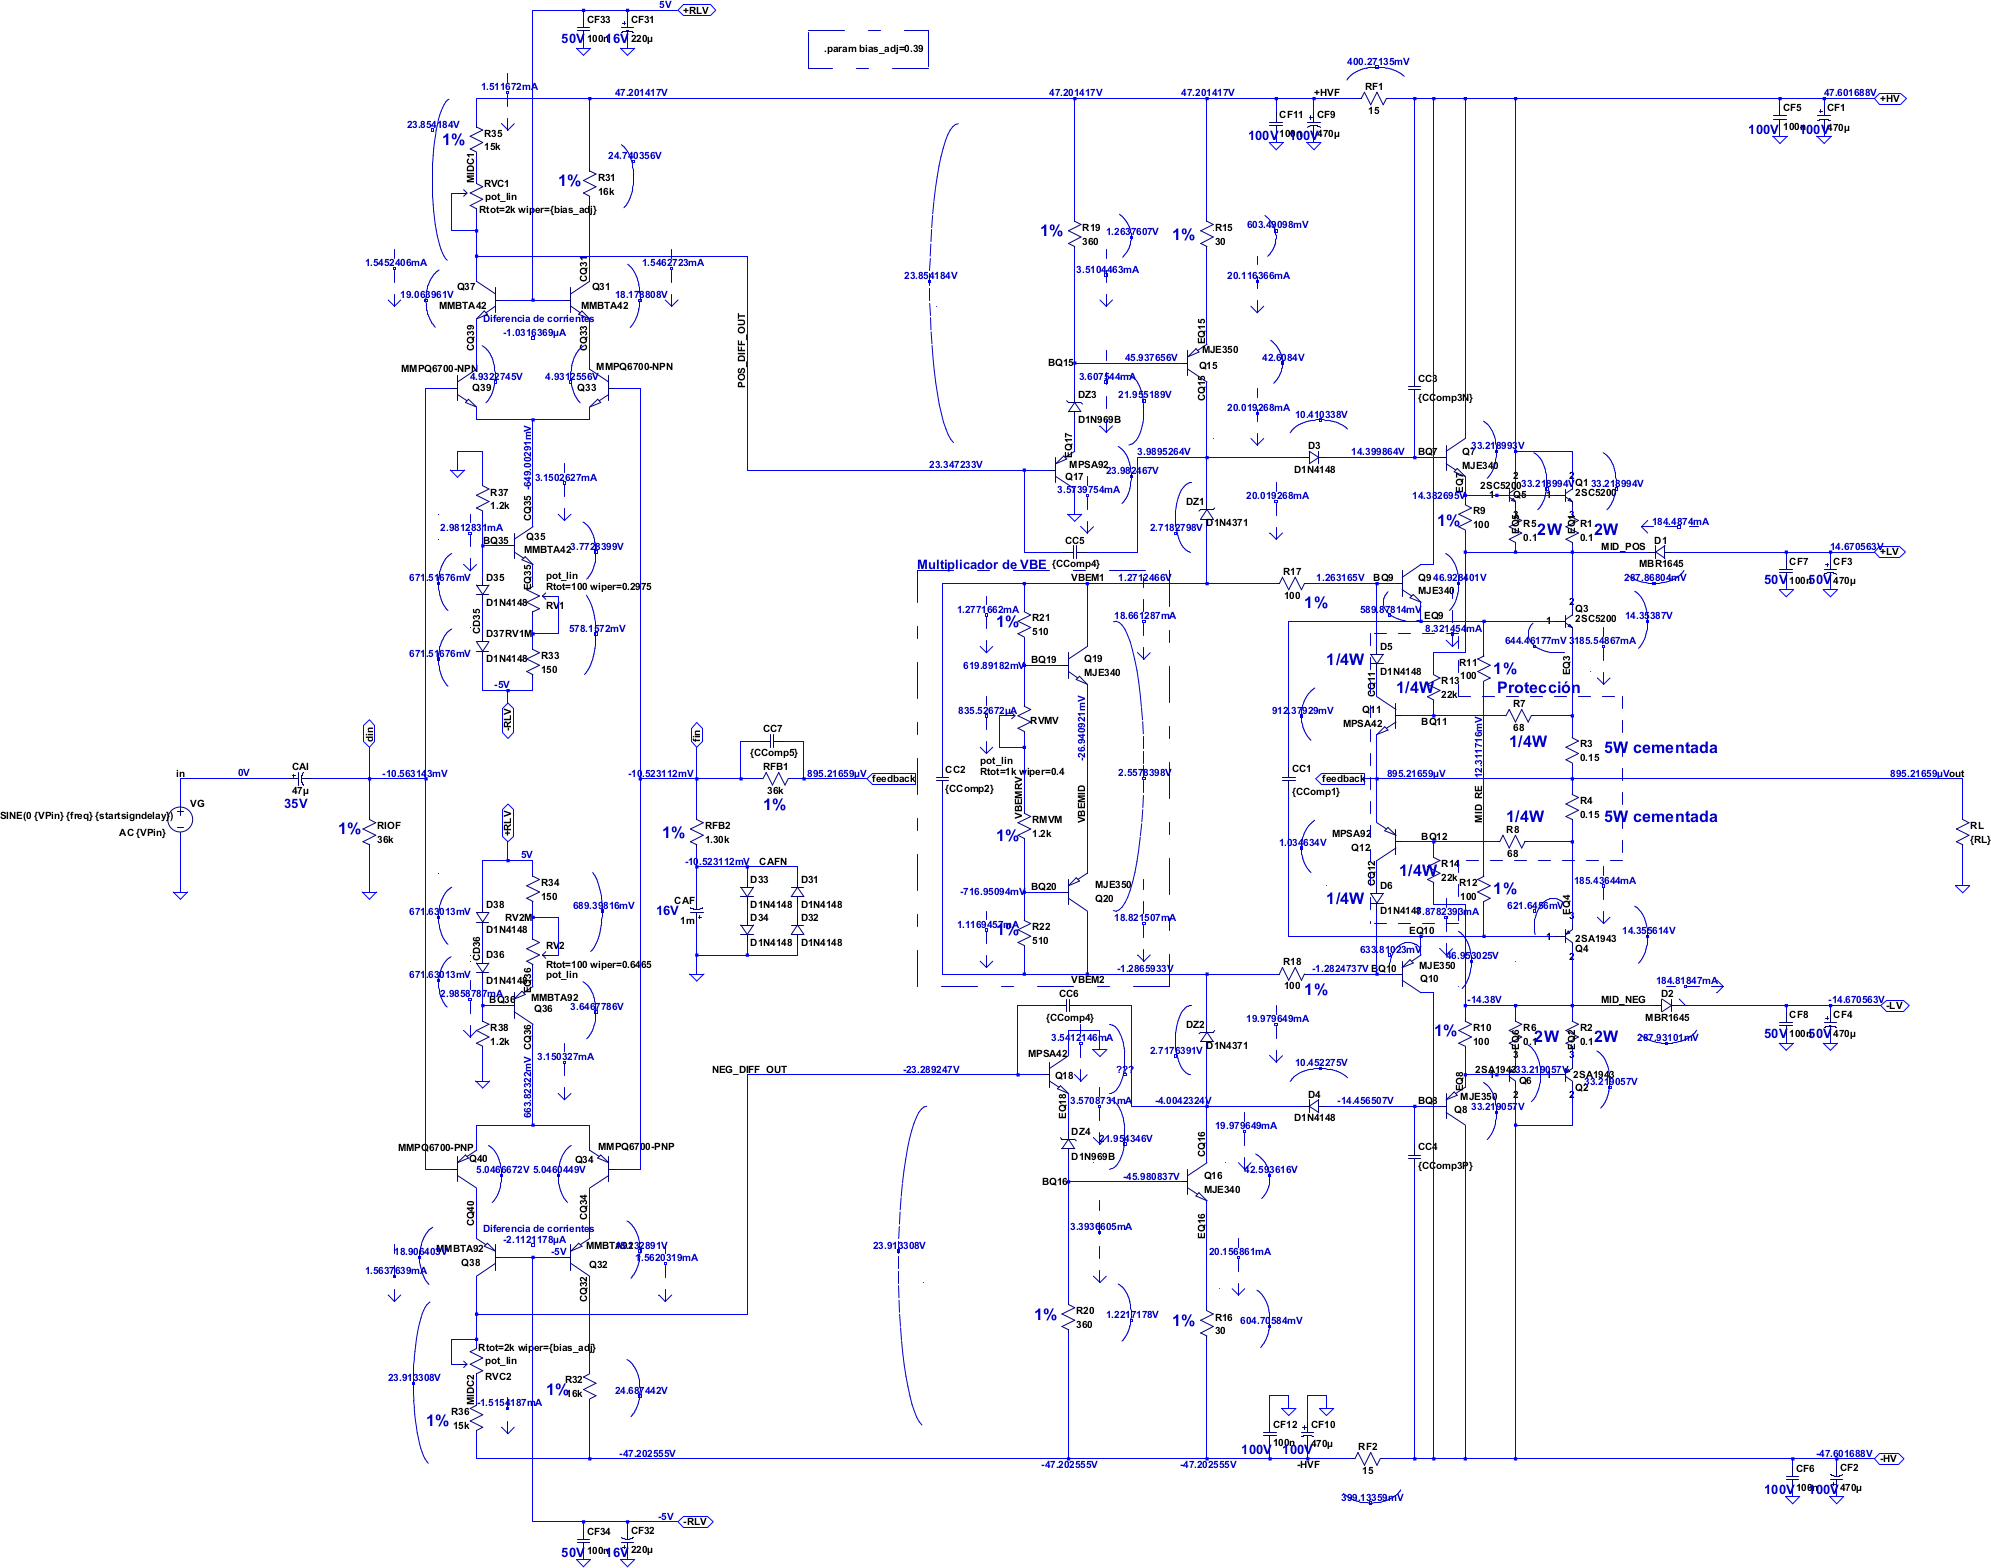
\includegraphics[width=0.9\paperwidth,angle=90,origin=c]{img/circuito.png}
\caption{Circuito Diseñado}
\label{fig:designed_circuit} 
\end{figure}

\clearpage


\subsection{Etapa de entrada}


Se usó doble par diferencial para mantener la simetría total y reducir la distorsión por armónicos pares, figura~\figref{fig:etapa-1}. Cada par se diseñó teniendo en cuenta que la tensión de salida de polarización debía ser estable, pues la segunda etapa no estará polarizada por una fuente de corriente. Por esto, los resistores de carga de los pares diferenciales ($R_{35}$, $RVC_{1}$ y $R_{36}$, $RVC_{2}$) son formadas por un resistor fijo de $15 \si[per-mode=symbol]{\kilo\ohm}$ y un preset multi-vuelta de $2 \si[per-mode=symbol]{\kilo\ohm}$, mucho menor que la resistencia dinámica de pequeña señal que le ofrece la segunda etapa ($\approx 60 \si[per-mode=symbol]{\kilo\ohm}$), dominando el paralelo. El ajuste de la polarización, consiste en ajustar primero la corriente de las fuentes de corriente y luego ajustar los presets de las cargas para lograr el punto deseado.
Por la misma razón, se consideró de particular importancia garantizar que las corrientes de polarización por las ramas del par se independicen de posibles variaciones en la segunda etapa o del riel. Los transistores $Q_{33}$~con~$Q_{39}$ y $Q_{34}$~con~$Q_{40}$, en configuración cascode combinados a $Q_{37}$~con~$Q_{31}$ y $Q_{38}$~con~$Q_{32}$ cumplen justamente la función de generar esta independencia.


\begin{wrapfigure}{R}{0.5\textwidth}
  \begin{center}
   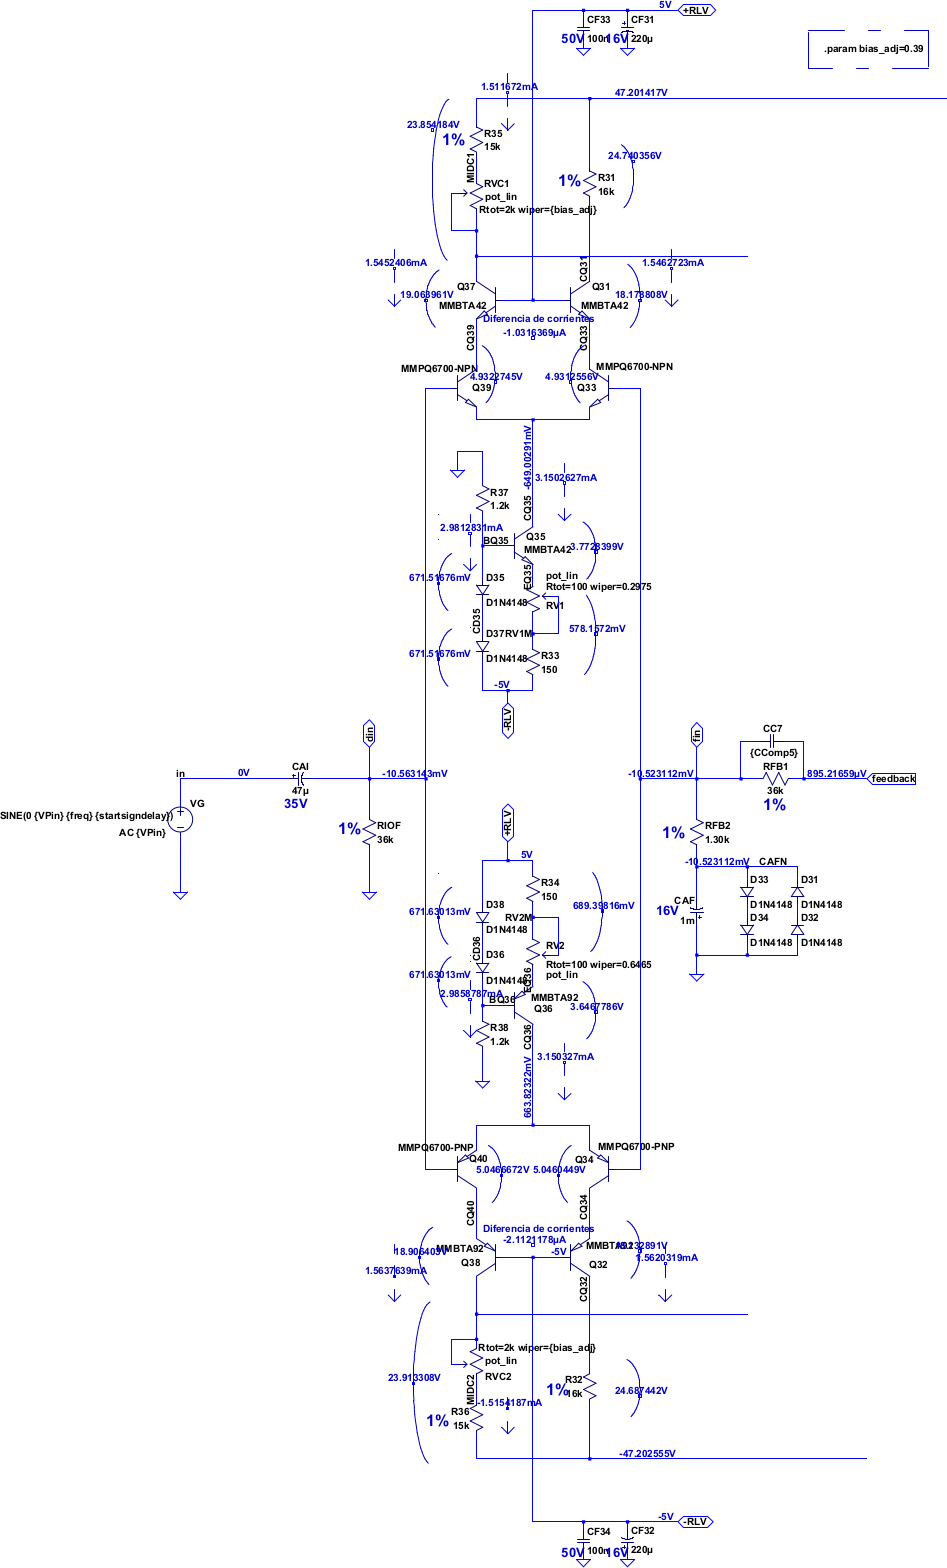
\includegraphics[width=0.4\textwidth]{img/etapa-1.png}
   \caption{Etapa primera del circuito diseñado.}
   \label{fig:etapa-1}
  \end{center}   
\end{wrapfigure}


Se polarizó cada rama con una corriente de $1.56 \si[per-mode=symbol]{\milli\ampere}$. Mayor corriente no generaría una mucho mayor amplificación de la etapa, pues, para mantener una tensión de salida fija habría sido necesario reducir la resistencia de carga en igual proporción. Esta corriente se generó con fuentes de corriente de $3.15 \si[per-mode=symbol]{\milli\ampere}$, se ajusta para que por los resistores de carga circulen $1.5 \si[per-mode=symbol]{\milli\ampere}$, logrando los $23.85 \si[per-mode=symbol]{\volt}$, independientes de la alimentación, que polarizan la segunda etapa. Los transistores de los pares diferenciales están formados cada uno por dos de los transistores de un array integrado, el \textbf{MMPQ6700}, de cuatro transistores, dos \textbf{NPN} y dos \textbf{PNP}, estos transistores como se mencionó tienen baja tensión de ruptura, pero el circuito elegido garantiza su operación segura, al ser integrados se tiene un grado alto de matcheo en sus características, esta característica se aprovecha para armar los diferenciales, dejando los base común de los cascodes a ser implementados por transistores complementarios discretos del tipo \textbf{MMBTA42}/\textbf{MMBTA92}, que son las versiones \textbf{SMD} de los conocidos transistores complementarios \textbf{MPSA42}/\textbf{MPSA92}, generalmente usados en amplificadores de potencia justamente por sus altas tensiones de ruptura y buenas características para audio.



%\begin{figure}[H]
%\centering
%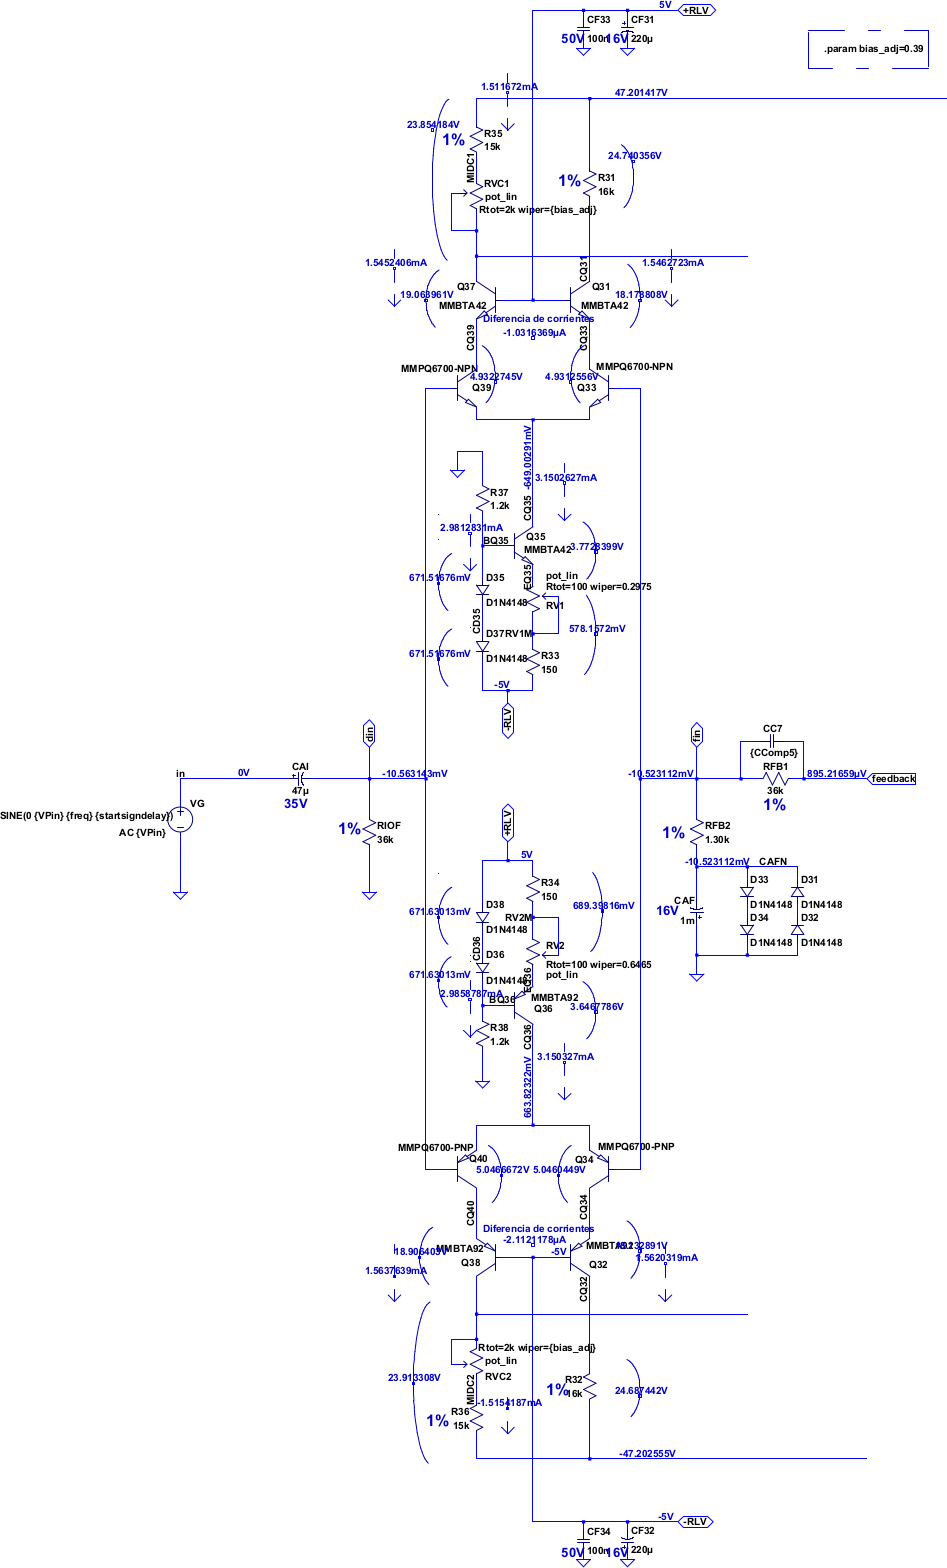
\includegraphics[width=0.36\textwidth]{img/etapa-1.png}
%\caption{Etapa primera del circuito diseñado.}
%\label{fig:etapa-1} 
%\end{figure}


\clearpage


\subsection{Etapa de amplificación de tensión}

Se optó por una configuración \textbf{CC-EC}, una para cada salida del doble par diferencial, figura~\figref{fig:vas-1}. El colector común cumple la función de ofrecer una resistencia alta a la primera etapa, independizando la polarización de los parámetros variables de los transistores de la segunda etapa. Además, aumenta la diferencia de tensión de polarización requerida entre el riel y la entrada de la etapa, lo que permite el uso de una resistencia de carga mayor en la primera etapa, mejorando su ganancia. Esta configuración, además, ofrece un alto grado de independencia de las variaciones de tensión del riel, pues todas las tensiones involucradas varían en conjunto (la única que no lo hace es masa, pero está conectada al colector de $Q_{17}$ y $Q_{18}$, nodos de alta impedancia). 


\begin{wrapfigure}{R}{0.5\textwidth}
  \begin{center}
   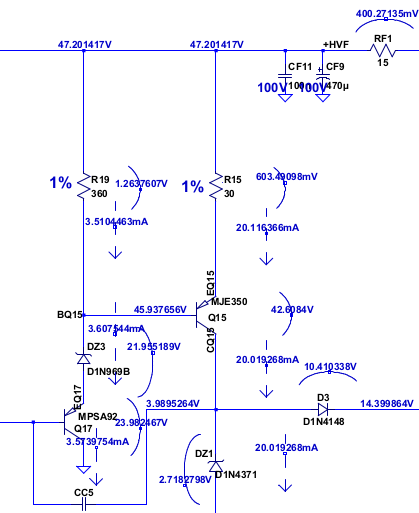
\includegraphics[width=0.4\textwidth]{img/vas-1.png}
   \caption{\textbf{VAS} en \textbf{CC-EC} del riel positivo del circuito diseñado (el otro \textbf{VAS} es perfectamente complementario).}
   \label{fig:vas-1} 
  \end{center}   
\end{wrapfigure}



%\begin{figure}[H]
%\centering
%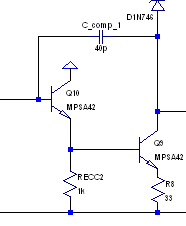
\includegraphics[width=0.3\textwidth]{img/sim/vas-1}
%\caption{VAS en CC-EC del riel negativo del circuito diseñado.}
%\label{fig:vas-1} 
%\end{figure}

Las resistencias de emisor de los \textbf{EC}, $R_{15}$ y $R_{16}$, implementan realimentaciones locales que estabilizan la corriente de polarización y ganancia de la etapa. Son realimentaciones \textbf{serie-serie} (muestrean corriente y suman tensión), estabilizando la transconductancia de la etapa. Son de valor reducido pues al estabilizar la ganancia, la reducen. Además, la caída de tensión en estas resistencias reduce la máxima excursión de la etapa antes de que saturen los transistores al mismo tiempo que determinan la corriente de colector. Se eligieron los valores exactos (junto con los de las cargas de la primera etapa) para que la corriente de polarización sea $20 \si[per-mode=symbol]{\milli\ampere}$.

Las resistencias $R_{19}$ y $R_{20}$ aseguran una corriente de polarización del colector común $3.5 \si[per-mode=symbol]{\milli\ampere}$. De no existir, la polarización podría ser muy baja, y dependiente de las variabilidades del $\beta$ del transistor del \textbf{EC}. Esta baja corriente implicaría, además, un $r_{d}$ grande, y esto es indeseable: El \textbf{EC} es un amplificador de conductancia y, como tal, funciona mejor recibiendo una señal de entrada de baja impedancia por su base.

Los transistores elegidos para los \textbf{VAS}, los complementarios \textbf{MJE340}/\textbf{MJE350}, de potencia media, que son lo mismos usados como drivers en la etapa de salida, fueron elegidos porque a pesar de que la corriente en esto transistores es moderada, su caída $V_{ce}$ es alta, haciendo que disipen potencias en el orden de $1 \si[per-mode=symbol]{\watt}$, estas potencias están fuera del rango adecuado para transistores de señal como son el par \textbf{MPSA42}/\textbf{MPSA92} utilizados en los seguidores, la potencia que disipan los pone justo en el límite de poder funcionar sin disipador, es posible que decidamos ponerles pequeños disipadores individuales a estos transistores.


En este punto es adecuado explicar el circuito pasa-bajos que se encuentra en los rieles de tensión alta que alimentan la primer y segunda etapa, estos simples pasa-bajos formados por un resistor y un par de capacitores, $RF_{1}$ con $CF_{9}$ y $CF_{11}$ en el riel positivo y $RF_{2}$ con $CF_{10}$ y $CF_{12}$ en el negativo, filtran el ripple de la fuente de alimentación (de $100 \si[per-mode=symbol]{\hertz}$), para eso el capacitor electrolítico de $470 \si[per-mode=symbol]{\micro\farad}$, que junto al resistor tienen una frecuencia de corte de $22.6 \si[per-mode=symbol]{\hertz}$, el capacitor cerámico de $100 \si[per-mode=symbol]{\nano\farad}$ está para filtrar el ruido de alta frecuencia que pueda filtrarse por los rieles de alimentación, principalmente debido a efectos causados por el switcheo de la etapa de salida. En general este filtrado reduce considerablemente el rechazo de de ripple de la fuente y también comprobamos que reduce un poco la distorsión, esto último es mas difícil de explicar.
Algo mas a mencionar de esta etapa, es que para adecuar la polarización del emisor común se utilizó en ambas ramas un zener de $22 \si[per-mode=symbol]{\volt}$, los mismos para la señal presentan a frecuencias medias solo una pequeña resistencia dinámica, por supuesto su capacidad parásita, afectará a altas frecuencias, pero las simulaciones indican que no perjudica al funcionamiento del circuito.

\clearpage


\subsection{Multiplicador de $V_{be}$}


El multiplicador de $V_{be}$ se diseñó con dos transistores, figura~\figref{fig:mvbe}, para mantener la simetría total del circuito y dado que, como ya se mencionó es adecuada para una etapa de salida con Darlingtons. La corriente de polarización de los transistores del VAS es $\cong 20 \si[per-mode=symbol]{\milli\ampere}$, y esta puede tener una excursión máxima de aproximadamente $4 \si[per-mode=symbol]{\milli\ampere}$ pico-a-pico. Es decir, el multiplicador debe lograr polarizarse con corrientes de $\cong 18 \si[per-mode=symbol]{\milli\ampere}$. Las simulaciones muestran que se logra una mayor estabilidad en la tensión si los transistores están polarizados con corrientes bajas. Por lo tanto, se eligió $RVMV$ tal que circule una corriente $< 19 \si[per-mode=symbol]{\milli\ampere}$, pero siempre del orden de los $\si[per-mode=symbol]{\milli\ampere}$. Se podría haber elegido un valor más cercano a $20 \si[per-mode=symbol]{\milli\ampere}$, pero una simulación remplazando al multiplicador por un generador de tensión ideal mostró que el funcionamiento y la distorsión del circuito no se veían afectados. 


\begin{wrapfigure}{R}{0.42\textwidth}
  \begin{center}
   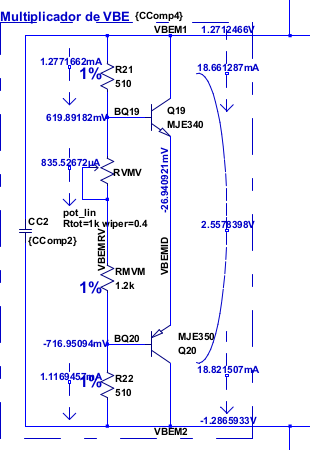
\includegraphics[height=0.5\textwidth]{img/mvbe.png}
   \caption{Multiplicador de $V_{be}$ simétrico utilizado.}
   \label{fig:mvbe}  
  \end{center}   
\end{wrapfigure}


Por esta misma razón, no se agregaron resistores adicionales en los colectores, que usualmente se usan para generar una caída que compense el incremento de tensión con la corriente. Puede hacerse como posible optimización.

Las resistencias $R_{21}$ y $R_{22}$ se eligieron iguales por simetría, y de valor tal que la tensión generada sea levemente superior a $2.5 \si[per-mode=symbol]{\volt}$. Esto permite colocar a los transistores de salida en modo levemente \textbf{A-B}, reduciendo la distorsión de su etapa.
De todas formas la manera de determinar en la práctica el valor adecuado de tensión del multiplicador, es ir aumentando la caída hasta que ya no baja la distorsión armónica, habiéndose eliminado por completo la distorsión de cruce por cero.\\
Los transistores utilizados son el par complementario \textbf{MJE340}/\textbf{MJE350}, los mismos de los VAS y drivers de la etapa de salida, son transistores de potencia media,  tienen encapsulado \textbf{TO-225}, adecuados para montar en un disipador, en este caso el motivo principal de su elección, ya que se podrían utilizar transistores de señal dado el nivel de disipación que tienen.



%\begin{figure}[H]
%\centering
%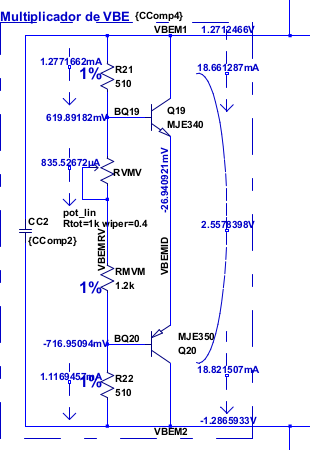
\includegraphics[height=0.5\textwidth]{img/mvbe.png}
%\caption{Multiplicador de $V_{be}$ simétrico utilizado.}
%\label{fig:mvbe} 
%\end{figure}


\clearpage



\subsection{Etapa de salida}

La etapa de salida, figura~\figref{fig:output_stage}, a pesar de parecer lo mas complicado, y ser lo primero que se diseña, es lo que menos problemas causó para determinar un circuito satisfactorio, es la única parte del circuito que no cambió a lo largo de las varias iteraciones del circuito global del amplificador, solo se le agregó el circuito de protección, del cual se probaron distintas configuraciones. Las simulaciones fueron muy satisfactorias con varios circuitos distintos en las primeras etapas, la elección correcta de los transistores de potencia fue crítica, y tener modelos proveídos por el fabricante ayudó a validar el diseño.
Se usan transistores en configuración Darlington, para tener una ganancia de corriente elevada, y con transistores en paralelo en los exteriores para repartir la corriente y disminuir la disipación en cada uno. Se colocaron los resistores $R_{1}$, $R_{5}$, $R_{2}$ y $R_{6}$ de valor $0.1 \si[per-mode=symbol]{\ohm}$ para ayudar a que se reparta de forma equilibrada la potencia entre los transistores de potencia $Q_{1}$-$Q_{5}$ y $Q_{2}$-$Q_{6}$ y estabilizarlos térmicamente, estos resistores se determinaron de $2\si[per-mode=symbol]{\watt}$, con lo cual se trata de resistores de carbón o metal de encapsulado un poco mayor al resto de los resistores de $0.25\si[per-mode=symbol]{\watt}$. Los transistores usados como drivers de los Darlington son los mismos para los internos como para los externos, se trata del par complementario \textbf{MJE340}/\textbf{MJE350}, el mismo utilizado en los VAS y el multiplicador de $V_{be}$, son de media potencia, con encapsulado \textbf{TO-225}, adecuados para poner en un disipador de ser necesario, estos transistores llevan un resistor de degeneración de emisor de $100 \si[per-mode=symbol]{\ohm}$, $R_{9}$ y $R_{10}$ para los drivers externos y $R_{11}$ y $R_{12}$ para los internos, algo interesante de estos resistores, es que en lugar de quedar conectados al punto de salida de conexión de la carga, se conectan uno con el otro salteando la conexión intermedia, esta configuración se observó en algunos circuitos comerciales simétricos, así como en el libro, las simulaciones demuestran que disminuye la distorsión armónica, aunque la explicación es difícil, aunque parece deberse a realimentación cruzada que solo es efectiva en estos circuitos completamente simétricos. 
Los transistores de salida $Q_{1}$-$Q_{5}$ y $Q_{2}$-$Q_{6}$, están todos formados por los pares complementarios \textbf{2SC5200}/\textbf{2SA1943} de la marca \textbf{Toshiba}, estos transistores de potencia, de encapsulado \textbf{TO-264}, están especialmente diseñados para amplificadores de potencia de hasta $100 \si[per-mode=symbol]{\watt}$, y son usados por \textbf{Toshiba} en sus propios amplificadores de potencia, son transistores de potencia rápidos, muy adecuados para una etapa clase G, tienen una corriente máxima de $15 \si[per-mode=symbol]{\ampere}$ y una tensión máxima de $V_{ce}$ de $230 \si[per-mode=symbol]{\volt}$. Los transistores de potencia internos necesitaban al igual que los externos unos resistores de degenaración de emisor de $0.1 \si[per-mode=symbol]{\ohm}$, sin embargo para que las protecciones limiten la corriente máxima a un valor alrededor de los $10 \si[per-mode=symbol]{\ampere}$, estos resistores se eligieron de $0.15 \si[per-mode=symbol]{\ohm}$ de $5 \si[per-mode=symbol]{\watt}$ del tipo de alambre cementado, los típicos bloques de color blanco, estos valores permiten soportar la máxima corriente por el tiempo necesario para que actúen las protecciones de la fuente de alimentación, en las condiciones normales de operación no disipan una potencia demasiado significativa, su principal perjuicio es aumentar la resistencia de salida del amplificador a lazo abierto.
El uso de los diodos Schottky \textbf{MBR1645}, el tipo de diodo, es simplemente debido a la baja caída que poseen, en el orden de $0.2 \si[per-mode=symbol]{\volt}$ para corrientes significativas, y el hecho que son rápidos, debido a no tener gran cantidad de carga acumulada como un diodo común, permitiendo que pasen rápidamente de conducción a cortados, el uso de ese específico diodo es debido a que no se observó diferencias con otros diodos similares, y se observó que estos en particular eran usados en varios circuitos comerciales, además de conseguirse fácilmente. Todos los rieles de alimentación altos y bajos, positivos y negativos para la etapa de potencia se encuentran filtrados por capacitores electrolíticos de $470 \si[per-mode=symbol]{\micro\farad}$, para filtrar el ripple y por capacitores cerámicos de $100 \si[per-mode=symbol]{\nano\farad}$ para compensar efectos inductivos que se traducen en señales de alta frecuencia que pueden afectar al circuito, especialmente las primeras etapas.


%\begin{wrapfigure}{L}{0.6\textwidth}
%  \begin{center}
%   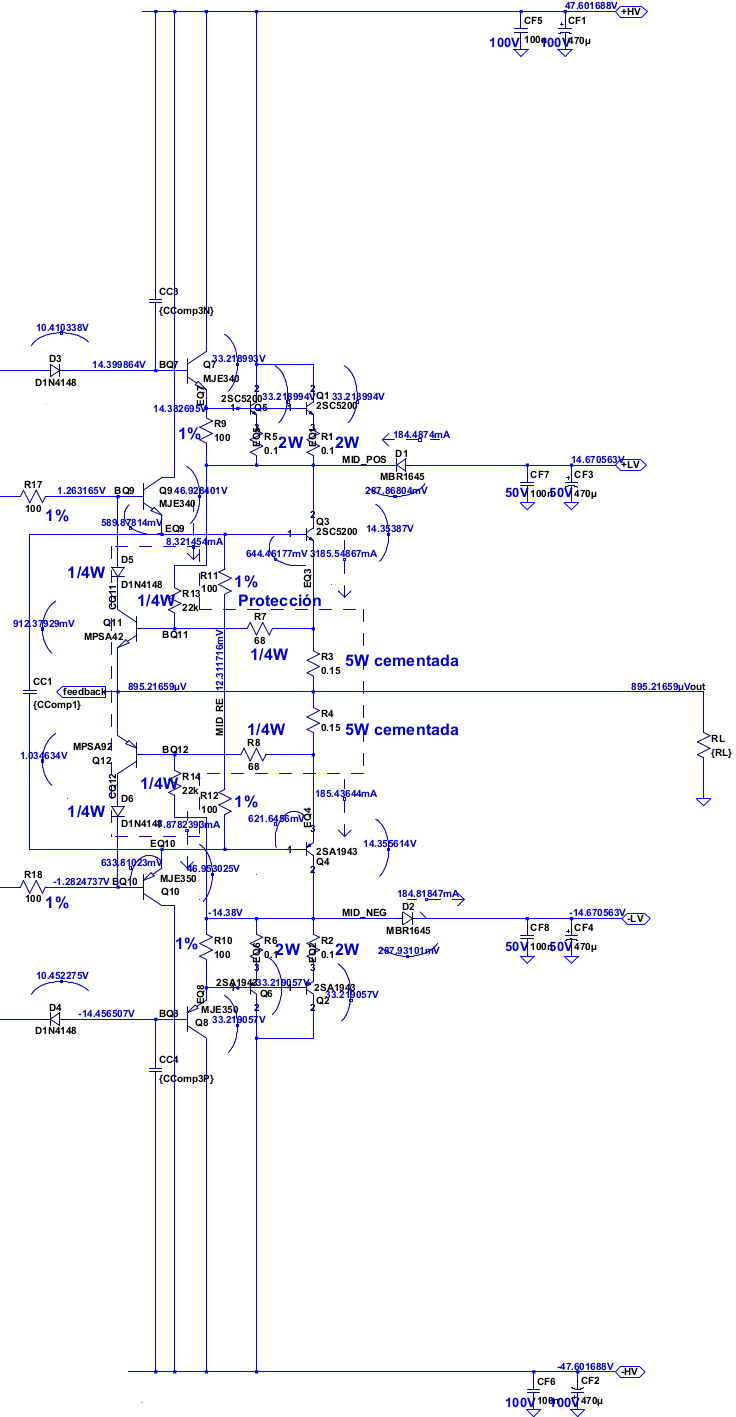
\includegraphics[height=0.5\paperheight]{img/output_stage.png}
%   \caption{Etapa de salida.}
%   \label{fig:output_stage}  
%  \end{center}   
%\end{wrapfigure}


\begin{figure}[H]
\centering
   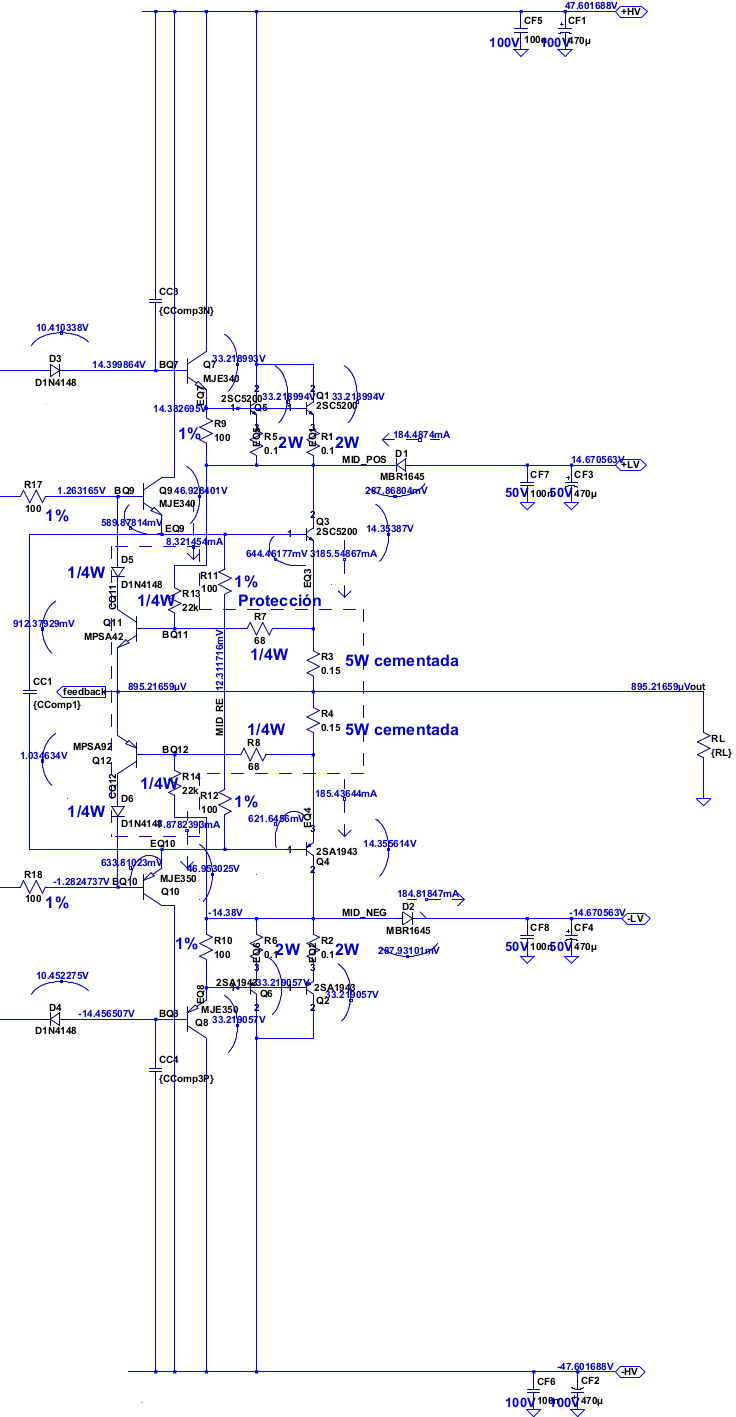
\includegraphics[height=0.66\paperheight]{img/output_stage.png}
   \caption{Etapa de salida.}
   \label{fig:output_stage}  
\end{figure}



\clearpage



\subsection{Realimentador}

Como se había mencionado en el diseño conceptual, el factor de realimentación queda definido por las especificaciones de sensibilidad y potencia RMS que definen la ganancia. Para nuestras especificaciones, la ganancia del amplificador debe ser de $29 \si[per-mode=symbol]{\decibel}$ y por lo tanto el realimentador debe atenuar $-29 \si[per-mode=symbol]{\decibel}$. Se implementa mediante un divisor de tensión que muestrea tensión y suma tensión. Deben ser resistencias lo suficientemente altas para que no afecten la salida al muestrear, y ya que para compensar el offset se usa un valor igual en la otra entrada de los diferenciales, uno de los resistores impone también la resistencia de entrada. Con una carga de $8 \si[per-mode=symbol]{\ohm}$, esto es sencillo. Por otra parte, la corriente que entra a la base del par diferencial de la primera etapa debe ser despreciable frente a la que circula por el realimentador para no afectar al factor $f$. Los valores usados se ven en la figura~\figref{fig:realimentacion-global}, los resistores se seleccionaron en valores cercanos a lo necesario dentro de los valores comerciales que se consiguen al $1 \si[per-mode=symbol]{\percent}$ de tolerancia, la tecnología seleccionada es metal film u oxide metal film, esto garantiza buena estabilidad con la temperatura y bajo ruido, cosa esencial en la red de realimentación.

\begin{figure}[H]
	\centering
	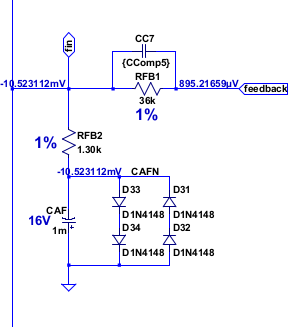
\includegraphics[width=0.4\textwidth]{img/realimentacion-global.png}
	\caption{Realimentación global implementada, junto con su compensación por atraso de fase.}
	\label{fig:realimentacion-global}
\end{figure}
 
 El capacitor $CAF$ cumple la función de modificar la realimentación en continua, a un factor unitario, y generar una simetría en las resistencias que ven las bases de los pares diferenciales de la primera etapa, y así reducir la tensión de offset. Por esta misma razón, la resistencia en paralelo a la entrada $RIOF$, que permite la polarización de $Q_{39}$ y $Q_{40}$ es del mismo valor que $RFB_{1}$.
 

Consideremos el diagrama de la figura~\figref{fig:ampli_realimentacion}. Para hallar los valores de impedancia de entrada y salida, primero debemos reflejar las resistencias $RFB_{1}$ y $RFB_{2}$, como vemos en el siguiente diagrama.

\begin{figure}[H]
	\centering
	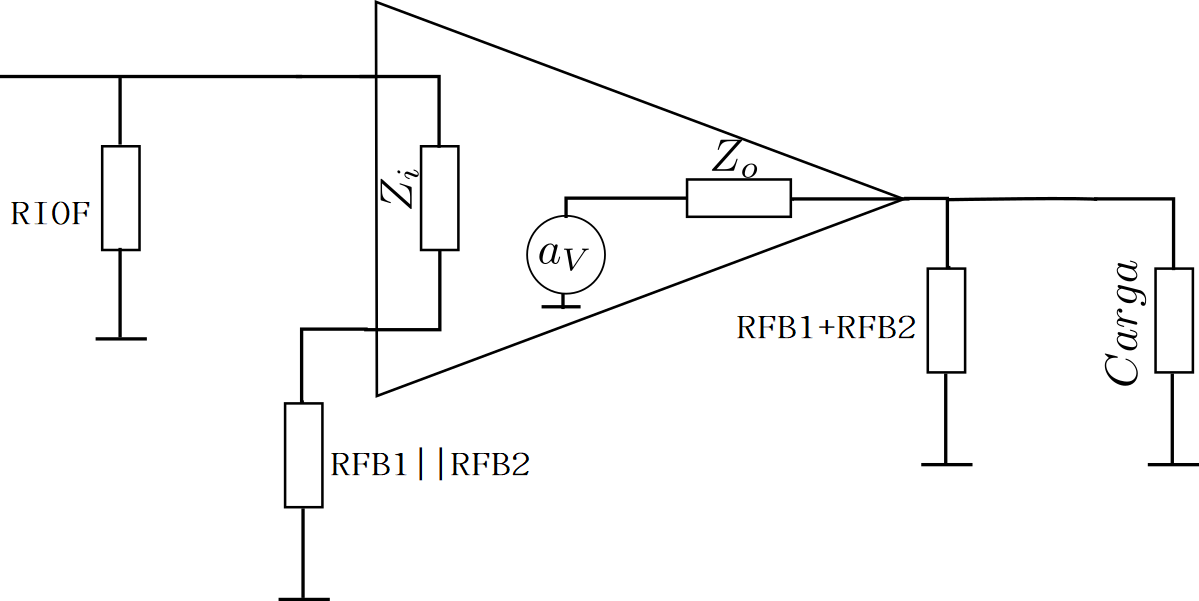
\includegraphics[width=0.5\textwidth]{img/reflejo.png}
	\caption{Modelo amplificador-reflejando resistencias}
	\label{fig:ampli_realimentacion}
\end{figure}


\begin{sloppypar}

Este amplificador tiene una amplificación de tensión a lazo abierto, de $76.35 \si[per-mode=symbol]{\decibel}$, con una impedancia de salida de aproximadamente $6 \si[per-mode=symbol]{\ohm}$.
La realimentación tiene un valor de ${ f = \frac{RFB_{2}}{RFB_{1} + RFB_{2}} \rightarrow f = 0.035 }$, resultando ${T = 1 + a_{V} \cdot f = 1 + 6569 \times 0.035 = 229.95}$. La ganancia a lazo cerrado es ${ A \cong \frac{1}{f} = 28.69 }$. En cuanto a la impedancia de entrada, $RFB_{1}$ y $RFB_{2}$ se reflejan en paralelo entre ellas, en serie a la impedancia de entrada del amplificador $Z_i$. Dada la relación entre las resistencias, $RFB_{1}$ resulta despreciable, y a su vez, $RFB_{2}$ resulta despreciable en serie con $Z_i$, que resulta despreciable, en paralelo con $RIOF$, de $36 \si[per-mode=symbol]{\kilo\ohm}$. Para la resistencia de salida, tenemos la resistencia reflejada $RFB_{1} + RFB_{2}$, que es despreciable en paralelo con $Z_o || R_{Carga} = 3.42 \si[per-mode=symbol]{\ohm}$. Luego ${ \frac{3.42}{(1 + a_{V} \times f)} = 0.01 \si[per-mode=symbol]{\ohm} }$, que es la impedancia de salida resultante. La impedancia de entrada incrementada en la ganancia de lazo resulta ser mucho mayor a $36 \si[per-mode=symbol]{\kilo\ohm}$. En nuestro circuito, la resistencia $RIOF$ de valor $36 \si[per-mode=symbol]{\kilo\ohm}$ en paralelo a la entrada del amplificador a lazo cerrado que domina la impedancia de entrada final.

\end{sloppypar}



\subsection{Compensación}

Un sistema realimentado puede sufrir de pérdidas de estabilidad debido al desfasaje que se produce en la señal. Si para algunas frecuencias se produce una inversión de fase y la ganancia es unitaria o mayor entonces el sistema pasa a estar realimentado positivamente para dichas frecuencias y oscila o se desestabiliza.

Para analizar la estabilidad del sistema es necesario analizar la ganancia a lazo abierto $T(j\omega)$. Un sistema adquiere la capacidad de oscilar si para una frecuencia dada $\omega_{k}$ se da que $T(j\omega_{k})=-1$ y se vuelve inestable si $\left| T(j\omega_{k}) \right| > 1 \; \land \; \angle T(j\omega_k) < -180 \si[per-mode=symbol]{\degree}$.

Para esta clase de análisis es útil trazar el bode de la ganancia de lazo e identificar el margen de ganancia (\textbf{MG}) y de fase (\textbf{MF}), ver figura \figref{fig:margenes}.


\begin{figure}[H]
	\centering
	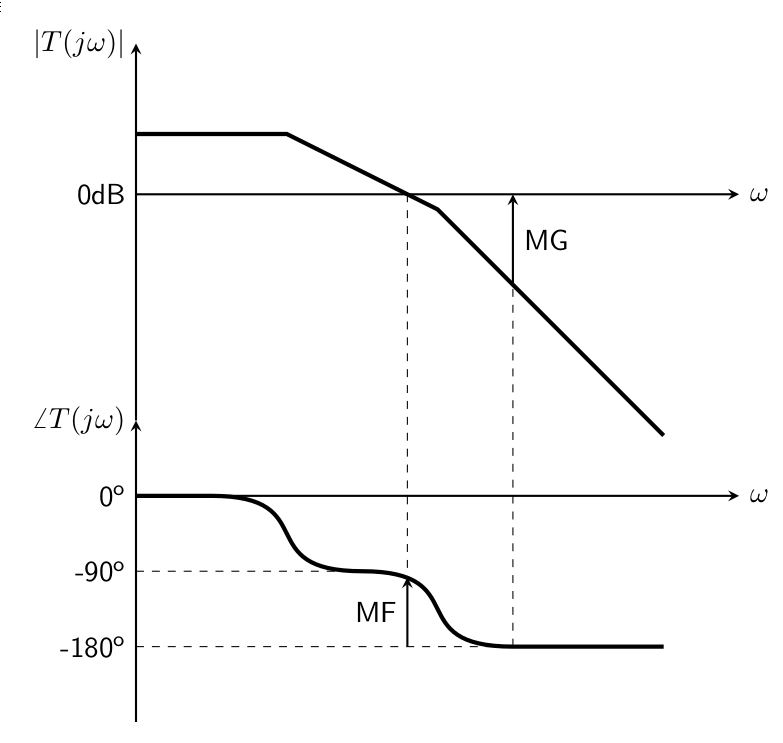
\includegraphics[height=0.35\textwidth]{img/margenes.png}
	\caption{Bode - margen de fase y ganancia.}
	\label{fig:margenes}
\end{figure}


Lo que representan estos margenes es lo siguiente:


\begin{description}
	\item[Margen de Ganancia] \hfill \\
		Representa la ganancia que habría que agregar (sumar en caso de $ \si[per-mode=symbol]{\decibel}$) para volver inestable al sistema, se mide entonces la diferencia entre $0 \si[per-mode=symbol]{\decibel}$ y la ganancia para la frecuencia en que la fase se invierte $180 \si[per-mode=symbol]{\degree}$. Si $\mathrm{MG} \le 0 \si[per-mode=symbol]{\decibel}$ entonces el sistema es inestable.

	\item[Margen de Fase] \hfill \\
		Es el desfasaje que habría que agregar al sistema para volverlo inestable, se mide entonces el ángulo que le resta a la fase por llegar a $ -180 \si[per-mode=symbol]{\degree}$ al tener ganancia unitaria.
\end{description}

Si el margen de fase o ganancia son muy bajos o negativos, es necesario corregir, modificar el circuito para que no haya una inversión de fase en ninguna frecuencias que se amplifique en el lazo, por medio de su compensación.


\begin{figure}[H]
	\centering
	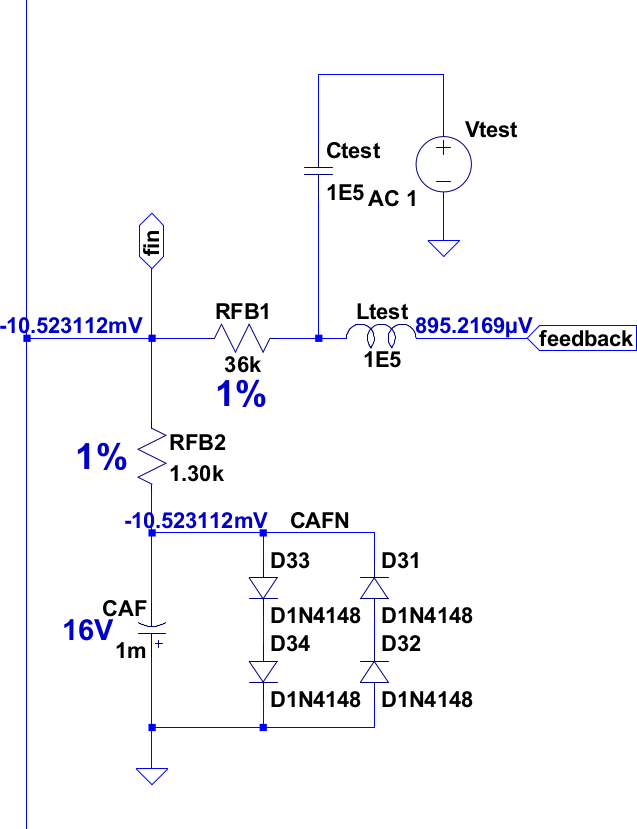
\includegraphics[height=0.35\textwidth]{img/sims/ala}
	\caption{Se abre el lazo anulando la realimentación en señal.}
	\label{fig:ala}
\end{figure}


Se realizó una simulación a lazo abierto, figura~\figref{fig:ala}, abriendo el lazo usando un capacitor y un inductor de valor grande. Luego se se midió la salida para obtener una simulación de la ganancia de lazo, figura~\figref{fig:bode-la-sin-comp}.




\clearpage

\begin{figure}[H]
	\centering
	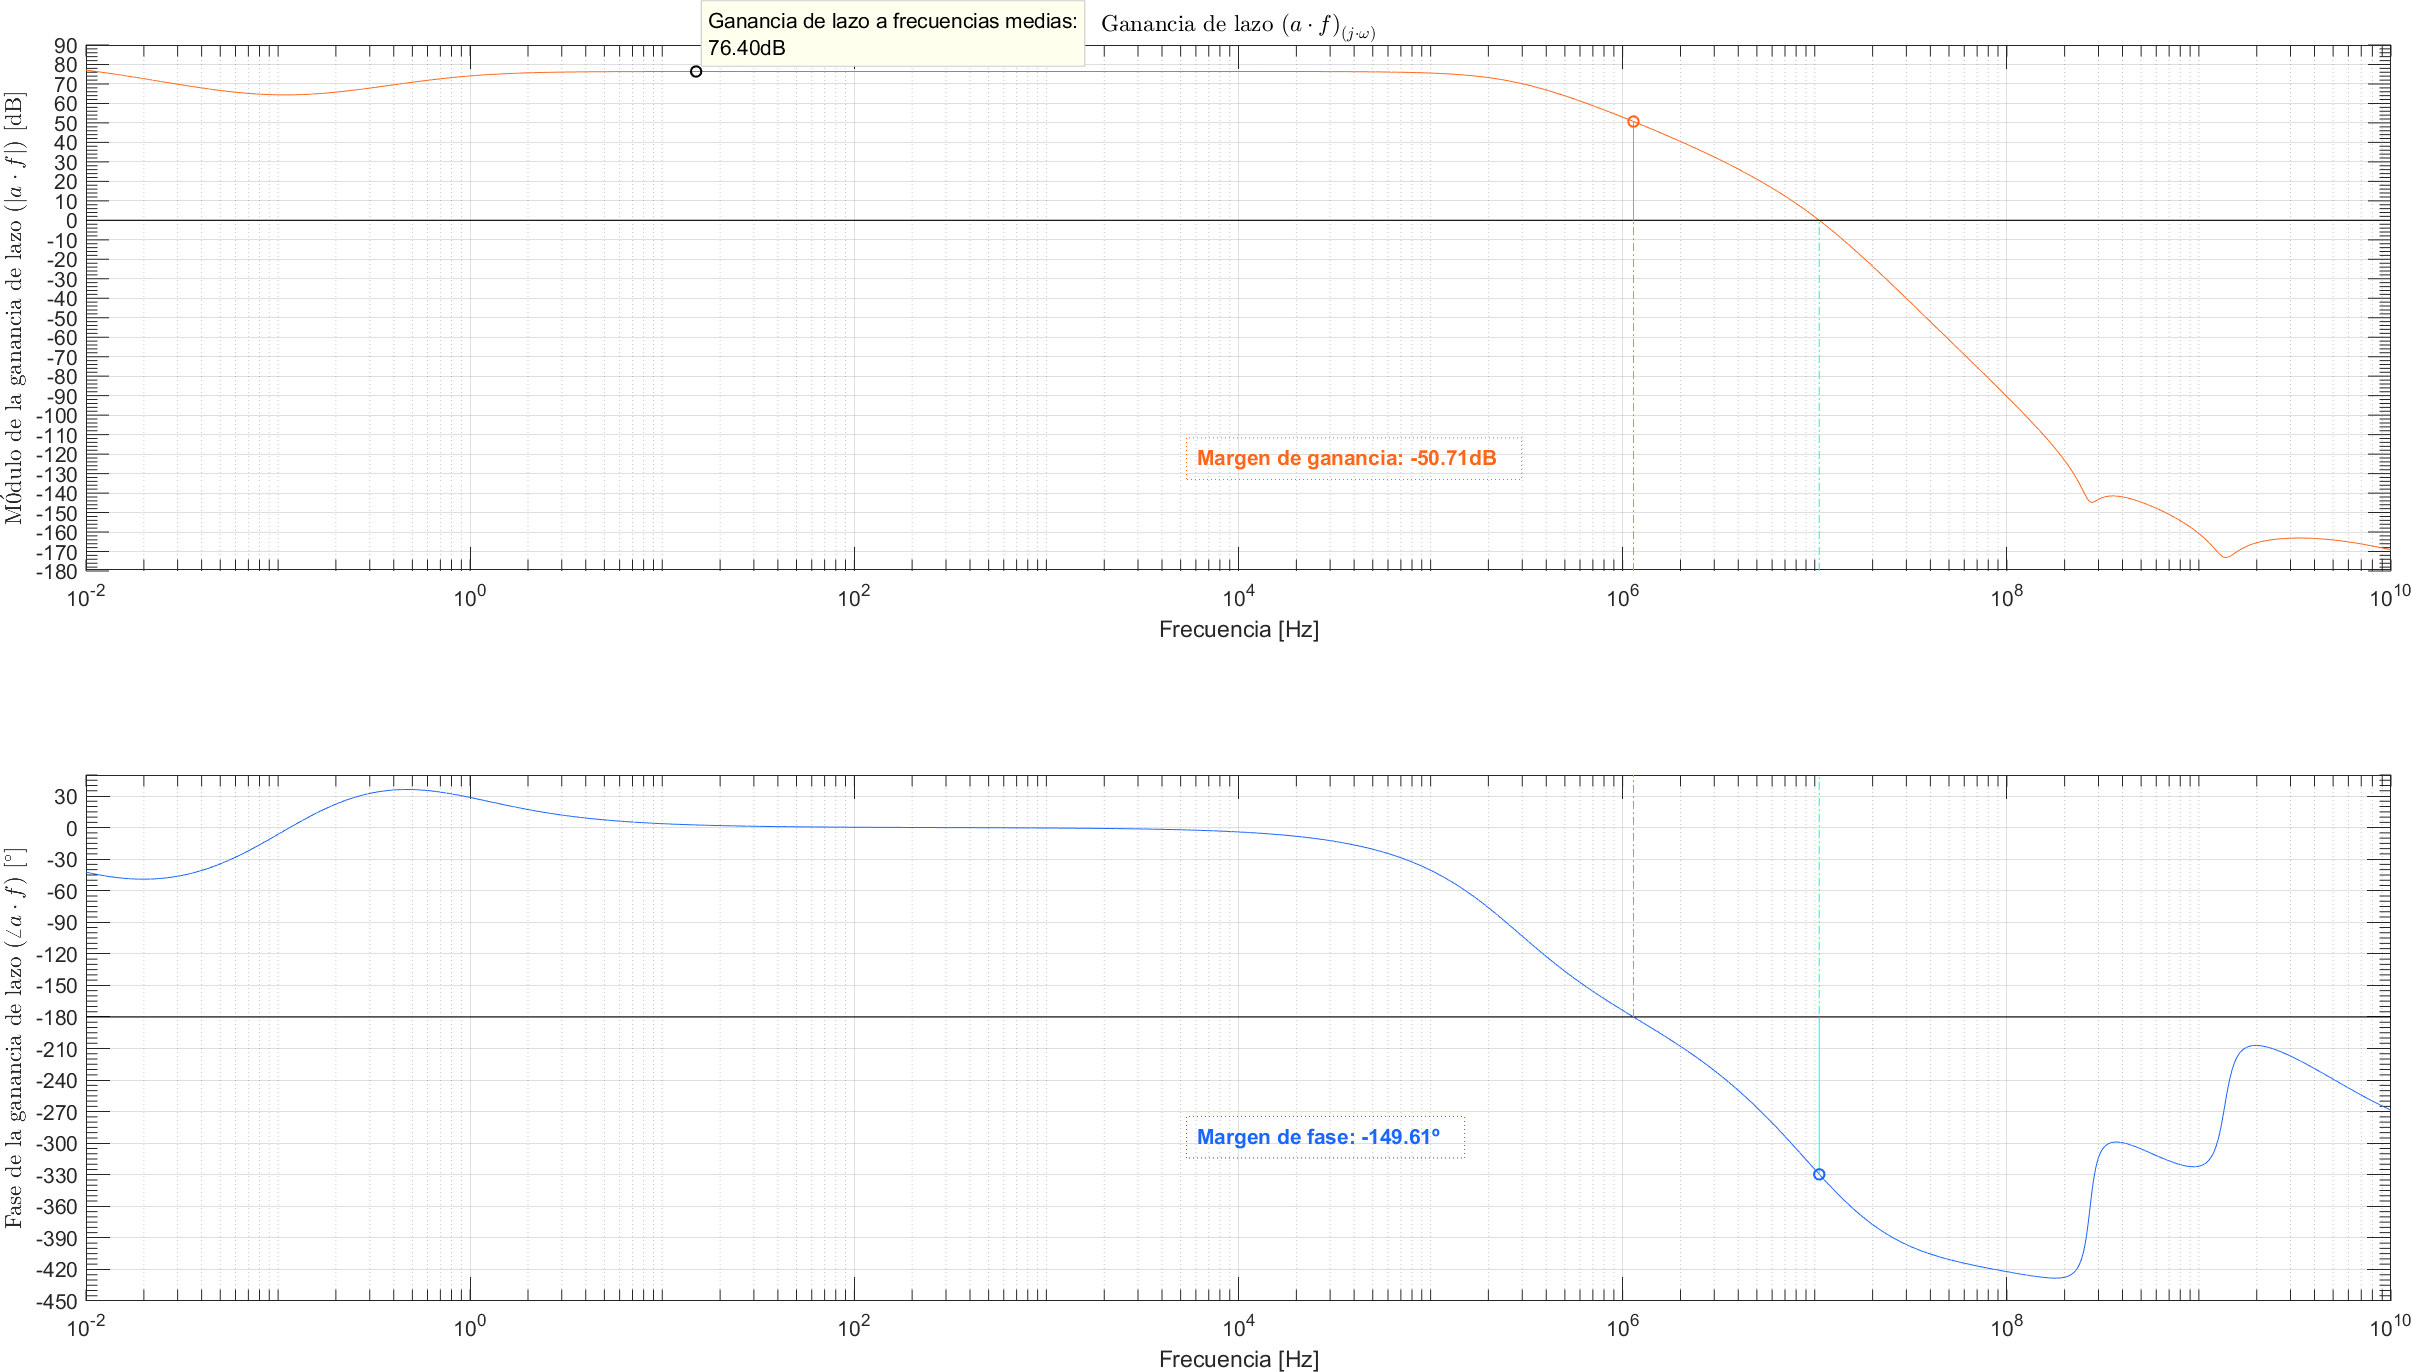
\includegraphics[width=0.85\paperwidth, angle=90]{img/sims/gain_loop_NC.png}
	\caption{Bode de la ganancia de lazo sin compensación.}
	\label{fig:bode-la-sin-comp}
\end{figure}

\clearpage



Se puede apreciar unos márgenes negativos que es necesario compensar. El polo dominante se ubica en aproximadamente $193 \si[per-mode=symbol]{\kilo\hertz}$ y corresponde al nodo entre la segunda y tercera etapa: a los colectores de $Q_{15}$ y $Q_{16}$. El margen de ganancia es de $\cong -50.7 \si[per-mode=symbol]{\decibel}$. Desplazando al polo dominante una década y media hacia las frecuencias más bajas (hasta $6.1 \si[per-mode=symbol]{\kilo\hertz}$) se llega a un margen de ganancia nulo, pues un polo hace decaer la ganancia en $20dB$ por década. Sin embargo, el polo correspondiente a los nodos de entrada de la segunda etapa (bases de $Q_{17}$ y $Q_{18}$) puede desplazarse a $6.1 \si[per-mode=symbol]{\kilo\hertz}$ con capacidades de menor valor, casi sin desplazar el polo en $193 \si[per-mode=symbol]{\kilo\hertz}$, aprovechando el efecto Miller. 
La resistencia de estos nodos está dominada por la de carga de los pares diferenciales ($RVC_{1} + R_{35}$ y $RVC_{2} + R_{36}$), de valor $16 \si[per-mode=symbol]{\kilo\ohm}$. Siendo $\frac{1}{2 \pi \cdot R \cdot C}$ la frecuencia del polo, se obtiene $C \cong 100 \si[per-mode=symbol]{\nano\farad}$. Ahora bien, si la capacidad se coloca, en vez de contra masa, contra la salida de la etapa (colectores de $Q_{15}$ y $Q_{16}$), se puede usar una capacidad desde $50 \si[per-mode=symbol]{\pico\farad}$, pues la etapa tiene una amplificación de alrededor de $62 \si[per-mode=symbol]{\decibel}$ o $1260$ veces. 

Se partió de ese valor como piso, se fue ajustando por simulación, y finalmente se colocaron capacitores ($CC_{5}$ y $CC_{6}$) de $100 \si[per-mode=symbol]{\pico\farad}$. Esto da un margen de fase de $80 \si[per-mode=symbol]{\degree}$ y un ancho de banda de $\cong 850 \si[per-mode=symbol]{\kilo\hertz}$. Estos capacitores limitan el Slew-Rate, pero se observó que para valores menores a $150 \si[per-mode=symbol]{\pico\farad}$ el Slew-Rate se encontraba por arriba de los $10 \si[per-mode=symbol]{\volt\per\micro\second}$ necesarios para el ancho de banda de potencia especificado, y para valores menores a $120 \si[per-mode=symbol]{\pico\farad}$, sobre los $15 \si[per-mode=symbol]{\volt\per\micro\second}$ especificados. Por otra parte, incrementar este capacitor reduce la ganancia de lazo en frecuencias altas y, por lo tanto, los beneficios que esto trae a la distorsión, resistencias de entrada y salida, etc. Se optó por un valor de capacidades, con margen, que podría eventualmente reducirse.

Luego, se agregó un capacitor en paralelo al realimentador ($CC_{7}$) para mejorar levemente estas especificaciones. Esto agrega un cero seguido de un polo. Por ejemplo, para la frecuencia del cero, la fase se incrementa en $45 \si[per-mode=symbol]{\degree}$ y la ganancia aumenta sólo en $3 \si[per-mode=symbol]{\decibel}$, por lo que el ancho de banda se verá incrementado levemente y el margen de fase significativamente. Se comprobó simulando que ubicar el cero en $4 \si[per-mode=symbol]{\mega\hertz}$ es un buen valor. Esto se obtiene con una capacidad de $1.2 \si[per-mode=symbol]{\pico\farad}$. El bode resultante de la ganancia de lazo compensado se muestra en la figura~\figref{fig:bode-la-con-comp}.


\clearpage

\begin{figure}[H]
	\centering
	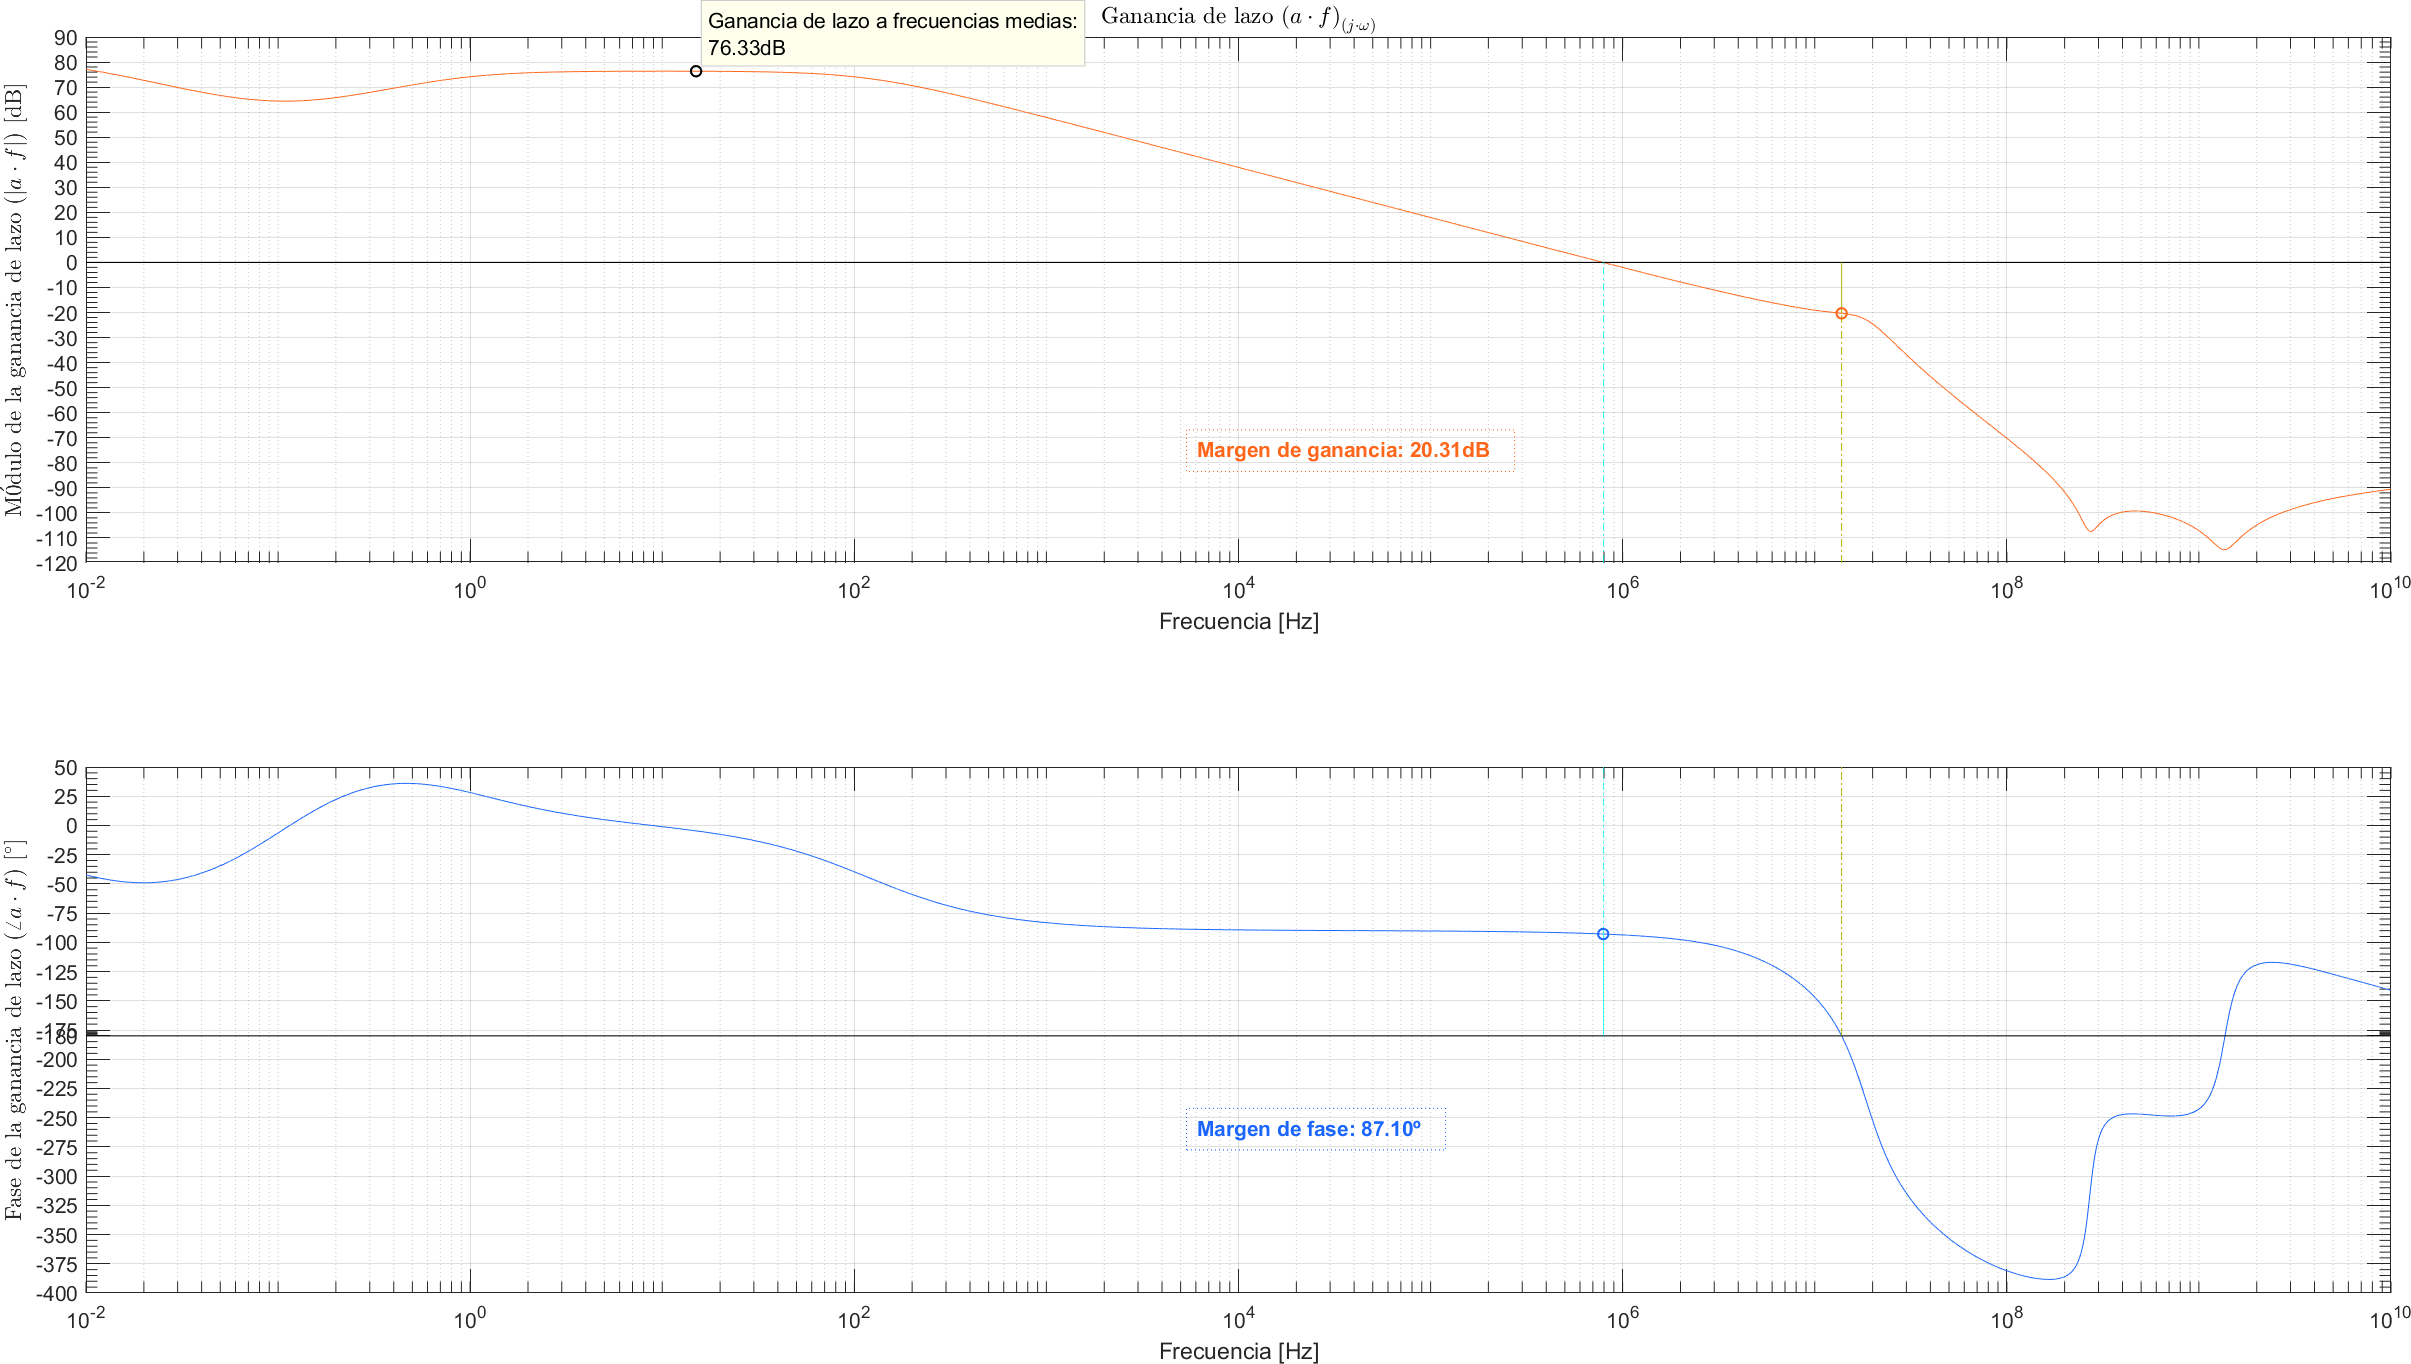
\includegraphics[width=0.85\paperwidth, angle=90]{img/sims/gain_loop_C.png}
	\caption{Bode de la ganancia de lazo compensado.}
	\label{fig:bode-la-con-comp}
\end{figure}

\clearpage


El margen de fase resultante ese de $87.1 \si[per-mode=symbol]{\degree}$ y el ancho de banda de $798 \si[per-mode=symbol]{\kilo\hertz}$, con un margen de ganancia de $20.3 \si[per-mode=symbol]{\decibel}$. Se puede ver en la figura~\figref{fig:slew} que la respuesta al escalón no oscila.

Se compensó el comportamiento inductivo del multiplicador de $V_{be}$ en altas frecuencias con el capacitor $CC_{2}$ de $6.8 \si[per-mode=symbol]{\nano\farad}$, su valor se halló simplemente aumentando el valor desde un valor de $1 \si[per-mode=symbol]{\nano\farad}$ hasta lograr una impedancia perfectamente plana en todo el ancho de banda, que luego cae monotonamente.

La última compensación, se trata de la compensación por alinealidad en la respuesta de los transistores de salida durante el switcheo, que puede verse claramente en las simulaciones, y es de alta frecuencia, esto se compensa colocando entre base y colector de los drivers externos los capacitores $CC_{3}$ y $CC_{4}$ de $68 \si[per-mode=symbol]{\pico\farad}$, valores hallados en forma empírica, y que probablemente requieran ajuste tras la medición del circuito armado.


Finalmente, con las ganancias a lazo abierto y lazo cerrado, realizamos el siguiente diagrama:

\begin{figure}[H]
	\centering
	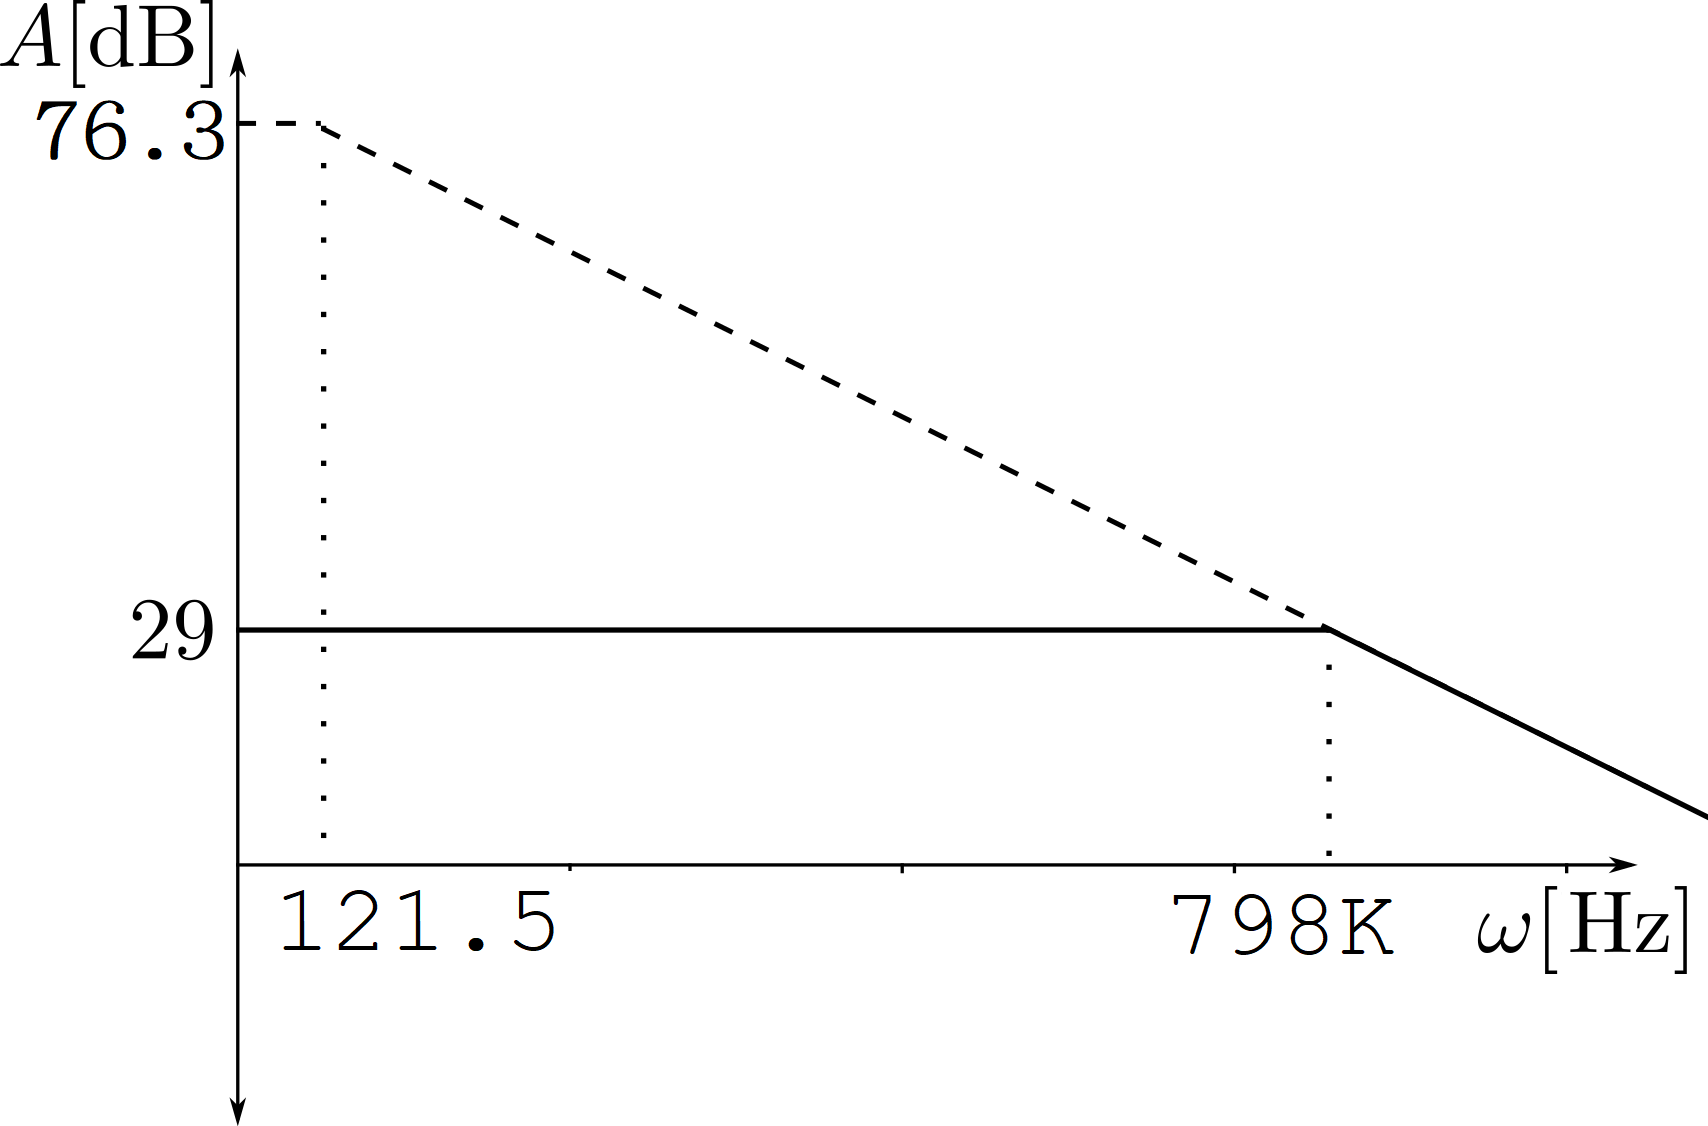
\includegraphics[width=0.5\textwidth]{img/bodecompensado.png}
	\caption{Aumento del ancho de banda, debido a la realimentación.}
	\label{fig:bode-compensado}
\end{figure}

Como se puede ver en el gráfico, la ganancia a lazo abierto, de $76.3 \si[per-mode=symbol]{\decibel}$, tiene un ancho de banda de $121.5 \si[per-mode=symbol]{\hertz}$, totalmente inútil para un amplificador de audio que trabaja con señales de decenas de $\si[per-mode=symbol]{\kilo\hertz}$. Cuando aplicamos la realimentación, la ganancia cae a $29 \si[per-mode=symbol]{\decibel}$, pero la frecuencia de corte pasa a ser $121.5 \si[per-mode=symbol]{\hertz} \times (1 + a_V \cdot f) = 122 \times 6569 = 798 \si[per-mode=symbol]{\kilo\hertz}$.